\chapter{Chemical Kinetic Mechanism Generation}
\section{Overview of Chemical Kinetic Mechanism}
Combustion at its very core, is an interdisciplinary field, that integrates the knowledge of physics of transport and reacting energy levels of species, the chemistry of reactions - rates of reactions (kinetics), fluid dynamics of flow fields, thermodynamics of reacting species based on energy levels both at the classical and statistical (quantum) levels and finally an appreciation of computer software and technology for computational analyses \cite{Curran2019DevelopingCombustion}. As a result of this interdisciplinary nature of the field, significant advances in each sub-discipline is virtually as important in bringing this field together in an age where technology is predominant and an ever increasing need to ensure the survival of the environment and human life, in quest to curb and understand negative effects of combustion, through air pollution from GHG as well as other emissions of harmful pollutants. 

Combustion is applied in almost all forms of daily life, that the understanding of each sub-discipline helps to further the current knowledge and appreciation of how well this field develops. From the very complex process of using internal combustion engines in automobiles, to the rotating shaft of turbines in both stationary gas turbines used in power plants and that of the aero-derivative gas turbines in airplane engines, to the industrial stove and gas burners to fertilizer and chemical processing and even HVAC systems. This plethora of applications has pushed an ever inquisitive solution to make these applications of combustion safer to humans and the environment as well as ensure the life cycle of devices that use these technologies. 

\begin{figure}

\centering
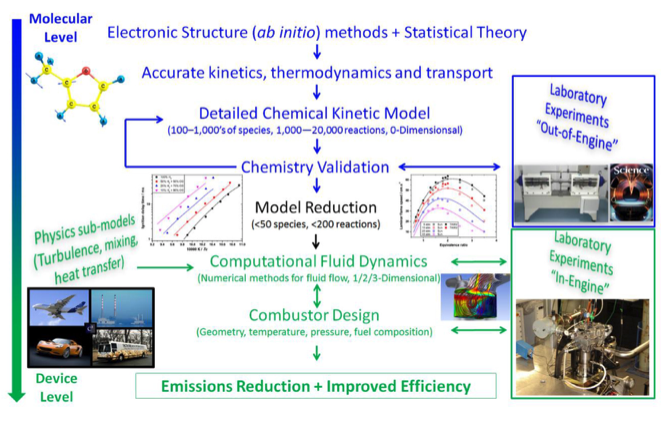
\includegraphics[scale=0.5, keepaspectratio]{images/combustion_schematic.png}
\caption{Schematic Diagram showing the different levels of understanding combustion from theory to application, courtesy of Dr.Kieran Somers \cite{Curran2019DevelopingCombustion}}
\label{fig:combustion_schematic}
\end{figure}

In fig.\ref{fig:combustion_schematic}, an ascending order of how combustion research starts off at :
\begin{enumerate}
        \item The molecular level with the need to understand species electronic structures using statistical theory and ab initio conditions, it includes those calculations of transitions states using quantum methods for reaction rates at intermediates and products used to quantify reacting species. This is the level where quantum methods are dominant and necessary for good estimates at level 2.
        \item Fuel structure and fundamental chemistry of fuel species, which is eventually stored in a database for kinetic, thermodynamic and transport parameters. This database is eventually used as a reference library to build detailed chemical kinetic models of a specific fuel or blends of fuels from elementary reactions using the reference libraries and database, based on the estimates from ab initio conditions of the thermo-kinetic parameters and validated with experimental measurements in homogeneous reactors for ignition-delay times, laminar flame speeds and species concentration profiles as well as rate of production/consumption of species.
        \item The reduction of the chemical kinetic mechanisms, which involves looking at the connection between reacting species and reactions through various methods like Sensitivity Analysis \cite{Rabitz1983SensitivityKinetics},\cite{Turanyi1990SensitivityApplications}, Directed Related Graph Method (DRG) \cite{Lu2005AReduction}, Directed Related Graph with Error Propagation (DRGEP)\cite{Pepiot-Desjardins2008AnMechanisms}, Directed Related Graph with Sensitivity-Analysis (DRGASA)\cite{Sankaran2007StructureFlame}\cite{Zheng2007Experimental13-butadiene}, Directed Related Graph with Error Propagation and Sensitivity Analysis (DRGEPSA) \cite{Niemeyer2010SkeletalAnalysis}, Computational Singular Perturbation \cite{Massias1999AnData}, Rate-Controlled-Reduced-Equilibrium methods (RCCE) \cite{Keck1971Rate-controlledMixtures}, which is done to reduce these kinetic mechanisms to only the core skeletal models of only a few hundred species with unimportant reactions and species removed for easy numerical computation of reactors and engines in CFD analysis that engine designers use.
        \item The last level is involved on practical applications, including policy regulation and efficiency of devices built especially the physical construction and building of these devices like internal combustion engines.
\end{enumerate}  

 So the link from molecular level to macro-level application is so enormous that most researchers typically focus on one or two levels at any given time. Level 2 is the of building detailed chemical kinetic models and exemplifies what this work is framed on for the purpose of GTL fuel surrogates. While, there will be mentions of level 1 during the course of the next chapters, level 2 entails the bulk of this thesis. 
 
 
\section{What is a Chemical Kinetic Mechanism ?}
 A chemical kinetic mechanism is numerical model that accurately contains the detailed elementary reactions of reacting species, thermodynamic estimates, associated rate constants with collider species, transport species at the specified reactor conditions of temperature, pressure and mole ratio \cite{Curran2019DevelopingCombustion}. This chemical kinetic mechanism can be very useful in describing reactions that are well known such as that of methane with oxygen described by the global reaction 
 
     \reaction{CH4 + 2O2 \longrightarrow CO2 + 2H2O}
 
 
 which really looks like a one-step reaction, however, contains about 200 elementary reactions and about 30 different species at a wide range of pressures and temperatures. Each elementary reaction describes the reactant and product species as well as the rate constant in both forward and reverse directions for a reversible reaction,
 
     \reaction{A\underset{k_r}{\stackrel{k_f}{\rightleftharpoons}}B}
  
 the forward rate constant $\ce{k_f}$ is often written as \ce{k_f[A]} while that of the reverse rate constant $\ce{k_r}$ is often written as \ce{k_r[B]}. This reaction rate constant is defined by the Arrhenius form defined as
 \begin{equation}
    k_f = A\times e^-{\frac{E_a}{RT}}
 \end{equation}
 \[\text{or that of the modified Arrhenius}\], 
 \begin{equation}
    k_f=A\times T^{\alpha}\times e^-{\frac{E_a}{RT}}
 \end{equation}
  At equilibrium, the forward and reverse rate constants are equal, thus
  \begin{equation}
  K_{eq}=K_c
  \end{equation}
  \[\text{also that} \]
  \begin{equation}
      K_{eq}=-\frac{\Delta G_r}{RT} 
  \end{equation}
  \[\text{and that}\]
  \begin{equation}
     K_c=\frac{k_f}{k_r}
  \end{equation}
  Then, at chemical equilibrium, 
  \begin{equation}
     K_{eq}=K_c=\frac{k_f}{k_r}
     \therefore K_{eq} = \frac{k_f}{k_r}
  \end{equation}
  
  and knowing that 
  \begin{equation}
    \Delta G_r = \Delta H_R -T\Delta S_R  
  \end{equation}
Where, $\Delta G_r$ is the Gibbs Free Energy of the reaction - indicating the energy available to do non-boundary (PV) work in a thermodynamically closed system at constant temperature and pressure and $\Delta H_R$ is the enthalpy of the reaction and $\Delta S_R$ is the entropy of the reaction. Thus, for reacting species, since the thermo-kinetic parameters of the forward rate constant is known, the corresponding reverse rate constant can be calculated from the equilibrium constant as a thermodynamic equilibrium is established. A chemical kinetic mechanism contains the thermo-kinetic parameters for the forward rate constants of elementary reactions at defined temperatures and pressures as well as the thermodynamic estimates and third body colliders. For flammability characteristics, the transport properties are also included in the mechanism.
 
 \section{Improvements in Chemical Kinetic Mechanisms}
 As a result of the complex reactions and reaction pathways involved in getting all possible elementary reactions and rate constants that describe many applicable reactions in combustion, the chemical kinetic modeling community has made significant improvements in the last three decades, with the development of various mechanisms aided with reaction pathways generated through automated computation, mechanisms such as the GRI-Mech\cite{Frenklach1995GRI-Mech---AnGRI-95/0058}\cite{BowmanGRI-Mech2.11}\cite{SmithGRI-Mech3.0} that was used to predict \ce{NOx} predictions and emissions of natural gas (methane),  Lawrence Livermore National Labs (LLNL) models of n-heptane and iso-octane as primary reference fuels of gasoline surrogates \cite{Curran1998AOxidation}\cite{Curran2002AOxidation}. As a result of the advances in computing technology, more complex models with more species and reactions have been built as seen in fig.\ref{fig:model_history} with carbon chains to \ce{C16} and \ce{C20}\cite{Westbrook2009AN-hexadecane}\cite{Sarathy2011ComprehensiveC20} and even oxygenated fuels \cite{Fischer2000TheReactors} as well as surrogate fuel models \cite{Mehl2011AnModelingb}. Recent strides have also been made towards the generation of jet fuel surrogate models \cite{Gokulakrishnan2008IgnitionFuel} \cite{Dooley2010AProperties}\cite{Mze-Ahmed2010KineticsStudy}\cite{Wang2012}\cite{Dagaut2014}\cite{Dagaut2014CombustionModeling}\cite{Narayanaswamy2016ASurrogates}\cite{Dagaut2016ExperimentalSurrogates}\cite{Singh2011ExperimentalFlames}. 
 
 \begin{figure}[hbp]
 \hspace*{-2cm}
     \centering
     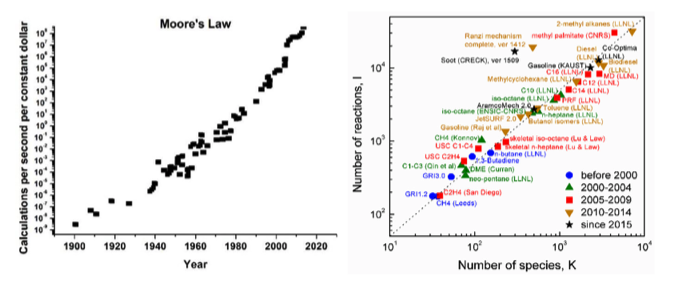
\includegraphics[scale=0.75,keepaspectratio]{images/model_history.png}
     \caption{Illustration of the correlation between computing power and mechanism size. Right hand side courtesy of Prof. Tianfeng Lu \cite{Curran2019DevelopingCombustion}}
     \label{fig:model_history}
 \end{figure}
 
 
 Most published kinetic models are validated with some uncertainty or error based on the estimates used, moreover since there exists no central database with which species estimation is benchmarked against save some experimental data or previous model, it is pertinent that a database be created not just for the estimation but also for the model generation of primary reference fuels for surrogates as well as comprehensive, detailed models of individual fuels validated against experiments such as ignition-delay times, laminar flame speeds and species concentration. Such database can be made into a library with easy access to determine where each model originates as well as how to construct more complex fuels based on the core mechanism of the \ce{C_0-C_4} chemistry. This quest for both a database library and automated model generation has birthed the use of more robust chemical kinetic mechanism software. 
 
 \section{Auotmated Chemical Kinetic Mechanism}
 The correlation between chemical kinetic mechanism and computing power has grown significantly over the years as seen in fig.\ref{fig:model_history} that it is almost impossible to attempt to build models without the aid the these numerical networks. As computing technology as improved as well as optimization of numerical methods, more models have been generated using automated software as well as interactive algorithms for the simulation of chemical mechanisms. The rise of Reaction Design's CHEMKIN suite originally developed by Sandia National Laboratories in the 1980's and now owned by ANSYS \cite{ANSYSCHEMKIN-PRO}, EXGAS \cite{Warth2000ComputerOxidation}, OPENSMOKE++\cite{Cuoci2015OpenSMOKE++:Mechanisms}\cite{Cuoci2013NumericalMethod}\cite{Stagni2014LumpingCoupling},LOGE-soft\cite{LOGESOFT}, Cantera\cite{cantera}, FlameMaster\cite{Pitsch1990FlameMasterCalculations}, CosiLab\cite{CosilabLaboratory}, CMCL Innovations kinetics\cite{ComputationalBuilder}, DETCHEM\cite{Deutschmann2019DETCHEMEd.},Chemical WorkBench\cite{Kintechlab:ChemicalWorkBench}, RMG\cite{Gao2016ReactionMechanisms}\cite{Allen2012AutomaticCoefficients}\cite{Magoon2013DesignGeneration}. These computer softwares are capable of generating chemical kinetic mechanism and validation of those mechanism with respect to some experimental measurement. There are four main capabilities needed for automatic chemical kinetic mechanism generators to possess to be able to be robust in the simulation of chemical species. They are:
 \begin{enumerate}
     \item A unique way to identify and represent chemical species correctly
     \item A method to determine what and how reactions can occur between chemically reacting species
     \item A means of getting good thermodynamic and kinetic estimates of parameters
     \item A criteria for inclusion or exclusion of species in the reaction model
 \end{enumerate}
     
 These numerical models continuously solve differential equations of the chemical reacting species based on some initial condition usually given or derived from experiments or boundary condition. The integration of these species is done by applying conservation laws of energy, mass, species and linear momentum for flame simulations within a given step size. As the integration continues, the time steps are adjusted for the next quantity estimating the temperature, pressure, velocity, species-concentration or mole fractions. The schemes used by most numerical solvers typically depend on the physical system being modeled, geometry, step-size and convergence criteria imposed. At any given time, if the time-step changes more faster than the solver scheme then it is bound to either fail or give incorrect approximations. As a result, most solvers are constrained to usually do uniform step-sizes as well as imposing a constant parameter to enable more efficient computation. 
 
 This work uses the reaction mechanism generator (RMG)\cite{Gao2016ReactionMechanisms}\cite{Allen2012AutomaticCoefficients}\cite{Magoon2013DesignGeneration} to construct three-component primary reference fuel (PRF) surrogate as a representation of GTL fuels. Each PRF consists of a detailed kinetic model with validations against experimental data. More emphasis is now laid on how RMG generates its models and the steps taken to build each PRF of n-decane, iso-octane and n-propyl-cyclohexane. 
 
 \newpage
 
 \section{Chemical Kinetic Mechanism Generation using Reaction Mechanism Generator (RMG)}
 \subsection{How RMG Works}
 RMG is an open-source software package that was developed at the Green Group at MIT to assist researchers and industry in the physical and chemical modeling of chemical reaction processes of elementary reactions. It is a Python based code of over 60,000 lines that also has the ability to calculate quantum estimates of species as well as at transition states.In addition, RMG has the unique capability of estimating transport properties for flamelet models and flammability analyses as well as solvation properties for liquid-phase species and automatically computes pressure-dependent rate constants and pressure-dependent rate networks for reaction flux analysis.
 
 RMG works on the framework of the general understanding of underlying reaction of elementary reactions and how they react. It employs the use of known chemistry methods stored in its library database from other chemical kinetic mechanisms along with its own unique property estimation methods to generate detailed chemical kinetic mechanisms. It relies primarily on two key principles: graph and tree structures to represent chemical species and represent both thermodynamic and kinetic parameters respectively. 
 
 Models are generated using a rate-based algorithm, which tracks the flux of species and excludes species based on the reaction flux criteria. RMG can generate mechanisms for species containing carbon, hydrogen, oxygen, sulphur and nitrogen \ce{C, H_2, O_2, S, N_2}.In order to construct a mechanism, an interactive script is first written for the specific set of species to be reacted as well as the reactor conditions for the reaction at initial conditions. Such conditions typically include temperature, pressure, species concentrations. RMG then takes the initial starting species and reacts all the species in all possible ways based on its own reaction families and then does a time integration of the model. 
 
 RMG tracks the rate of production of species as well as reactions at the edge (outside the initial starting species). As the reactions occur, the rate of production of new species and reactions outside the initial starting species grows with significance, the new reactions and species produced from further reaction is then added to the core of the initial starting species and the model grows bigger in size. As the new core species are then reacted with all other new species in the core thus, generating much species and reactions.As the time integration restarts, the list of edge species are tracked to determine which species will be added again to the core. This process continues until all the significant species are added to the core. A significant rate can be specified by the user, by using the following definition: 
 \begin{equation}
     R_i=\frac{dC_i}{dt}
 \end{equation}
 When the flux (rate of production of species) in the edge is greater than that of the characteristic species, it is moved to the core. The reaction system characteristic rate is the sum of the all core species rates, defined as:
 \begin{equation}
     R_{char}=\sqrt{\sum_j {R_{j}^2}} \hspace{1cm} \text{species j $\epsilon$ core}
 \end{equation}

 
 \begin{figure}[htp]
     \centering
     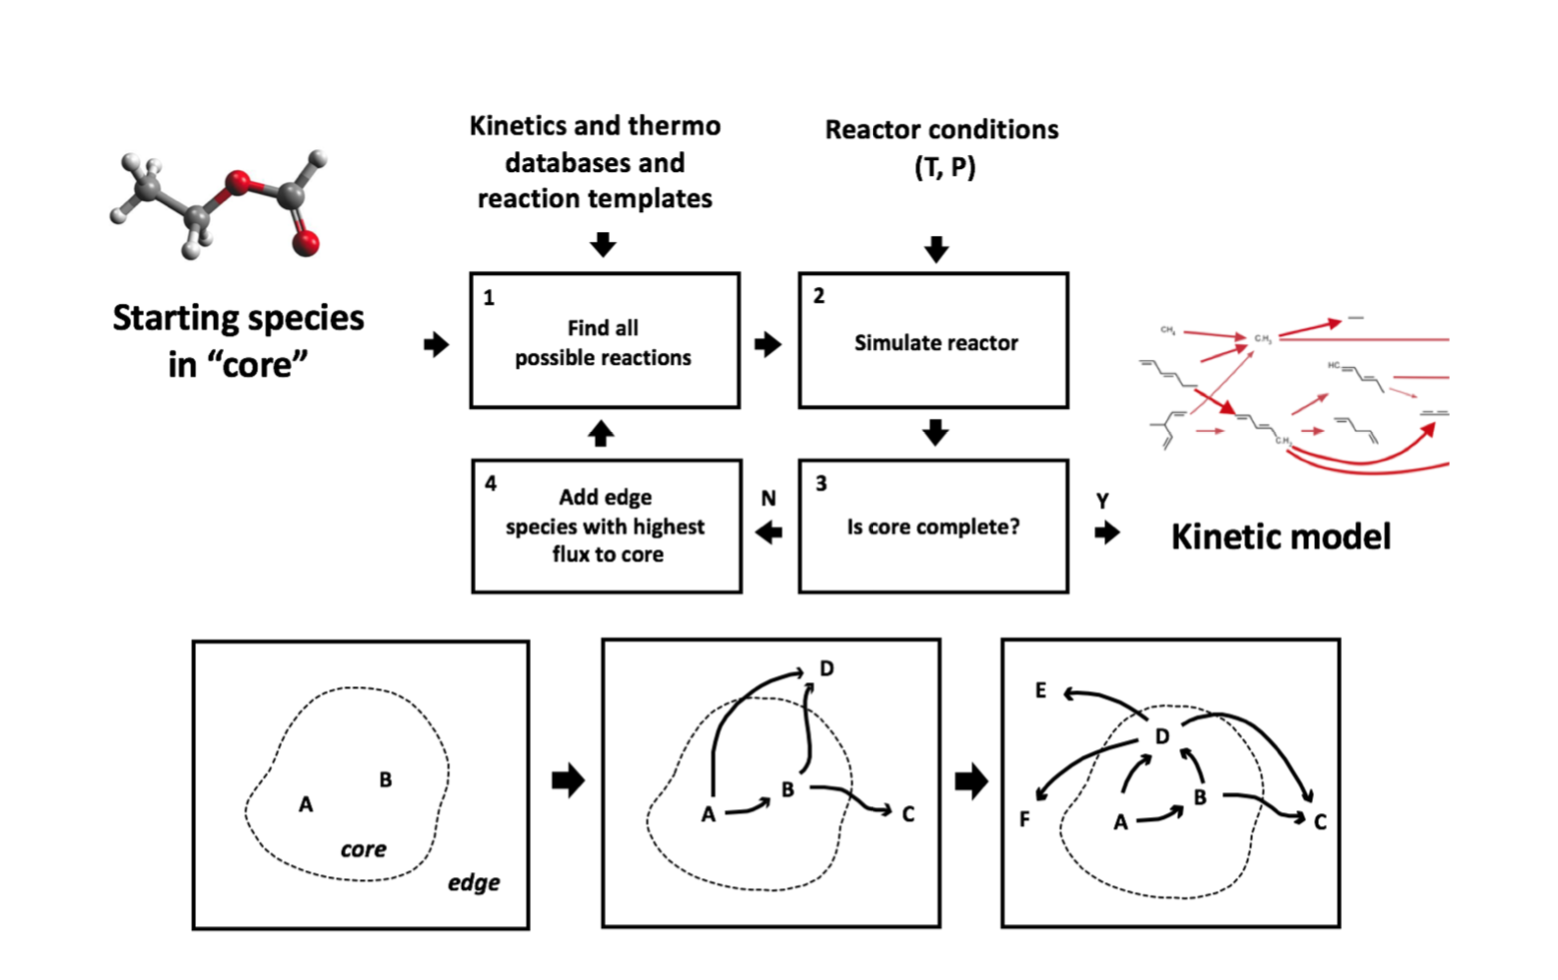
\includegraphics[scale=0.4,keepaspectratio]{images/rmg_core_build.png}
     \caption{RMG Rate-based Model Englarging Algorithm Schematic \cite{Susnow1997Rate-BasedSystems}\cite{Gao2016ReactionMechanisms}}
     \label{fig:rmg_core_build}
 \end{figure}
 
 RMG utilizes a functional group based algorithm to work with species and reactions. It is applied in such a way that each reactions family is defined by a set of templates that match functional groups as they go from reactants to products\cite{Gao2016ReactionMechanisms}. Chemical graph theory is applied for representing molecules as well as functional group substructures, with vertices indicating atoms while edges are used to indicate bonds.
 
 \subsection{RMG Thermodynamic Estimation}
 Species thermochemistry is estimated using Benson group additivity methods \cite{Benson1958AdditivityProperties}\cite{Benson:452788}for thermochemical parameters, such as enthalpy $\Delta H_f^{\circ}$, entropy $S^{\circ}$ and heat capacities $c_p$. For free radical, the hydrogen bond increment (HBI) method of Lay et al is applied \cite{Lay1995HydrogenSpecies}. RMG utilizes hierarchical trees to organize functional groups for ease of group identification. Trees structures are organized in such a way that the general functional groups are placed at the top nodes, then more specific functional groups are placed in the successive lower nodes.  Before thermodynamic estimates are computed, resonance structures of those species are run and obtained including non-straight chain (aromatic) structures of the species. The algorithm then checks for the presence of radicals in any of the resonance structures, which if present the HBI correction is applied, before proceeding to check for the contribution of the enthalpies, entropies and heat capacities of the saturated species. .
 \begin{figure}[ht]
     \centering
     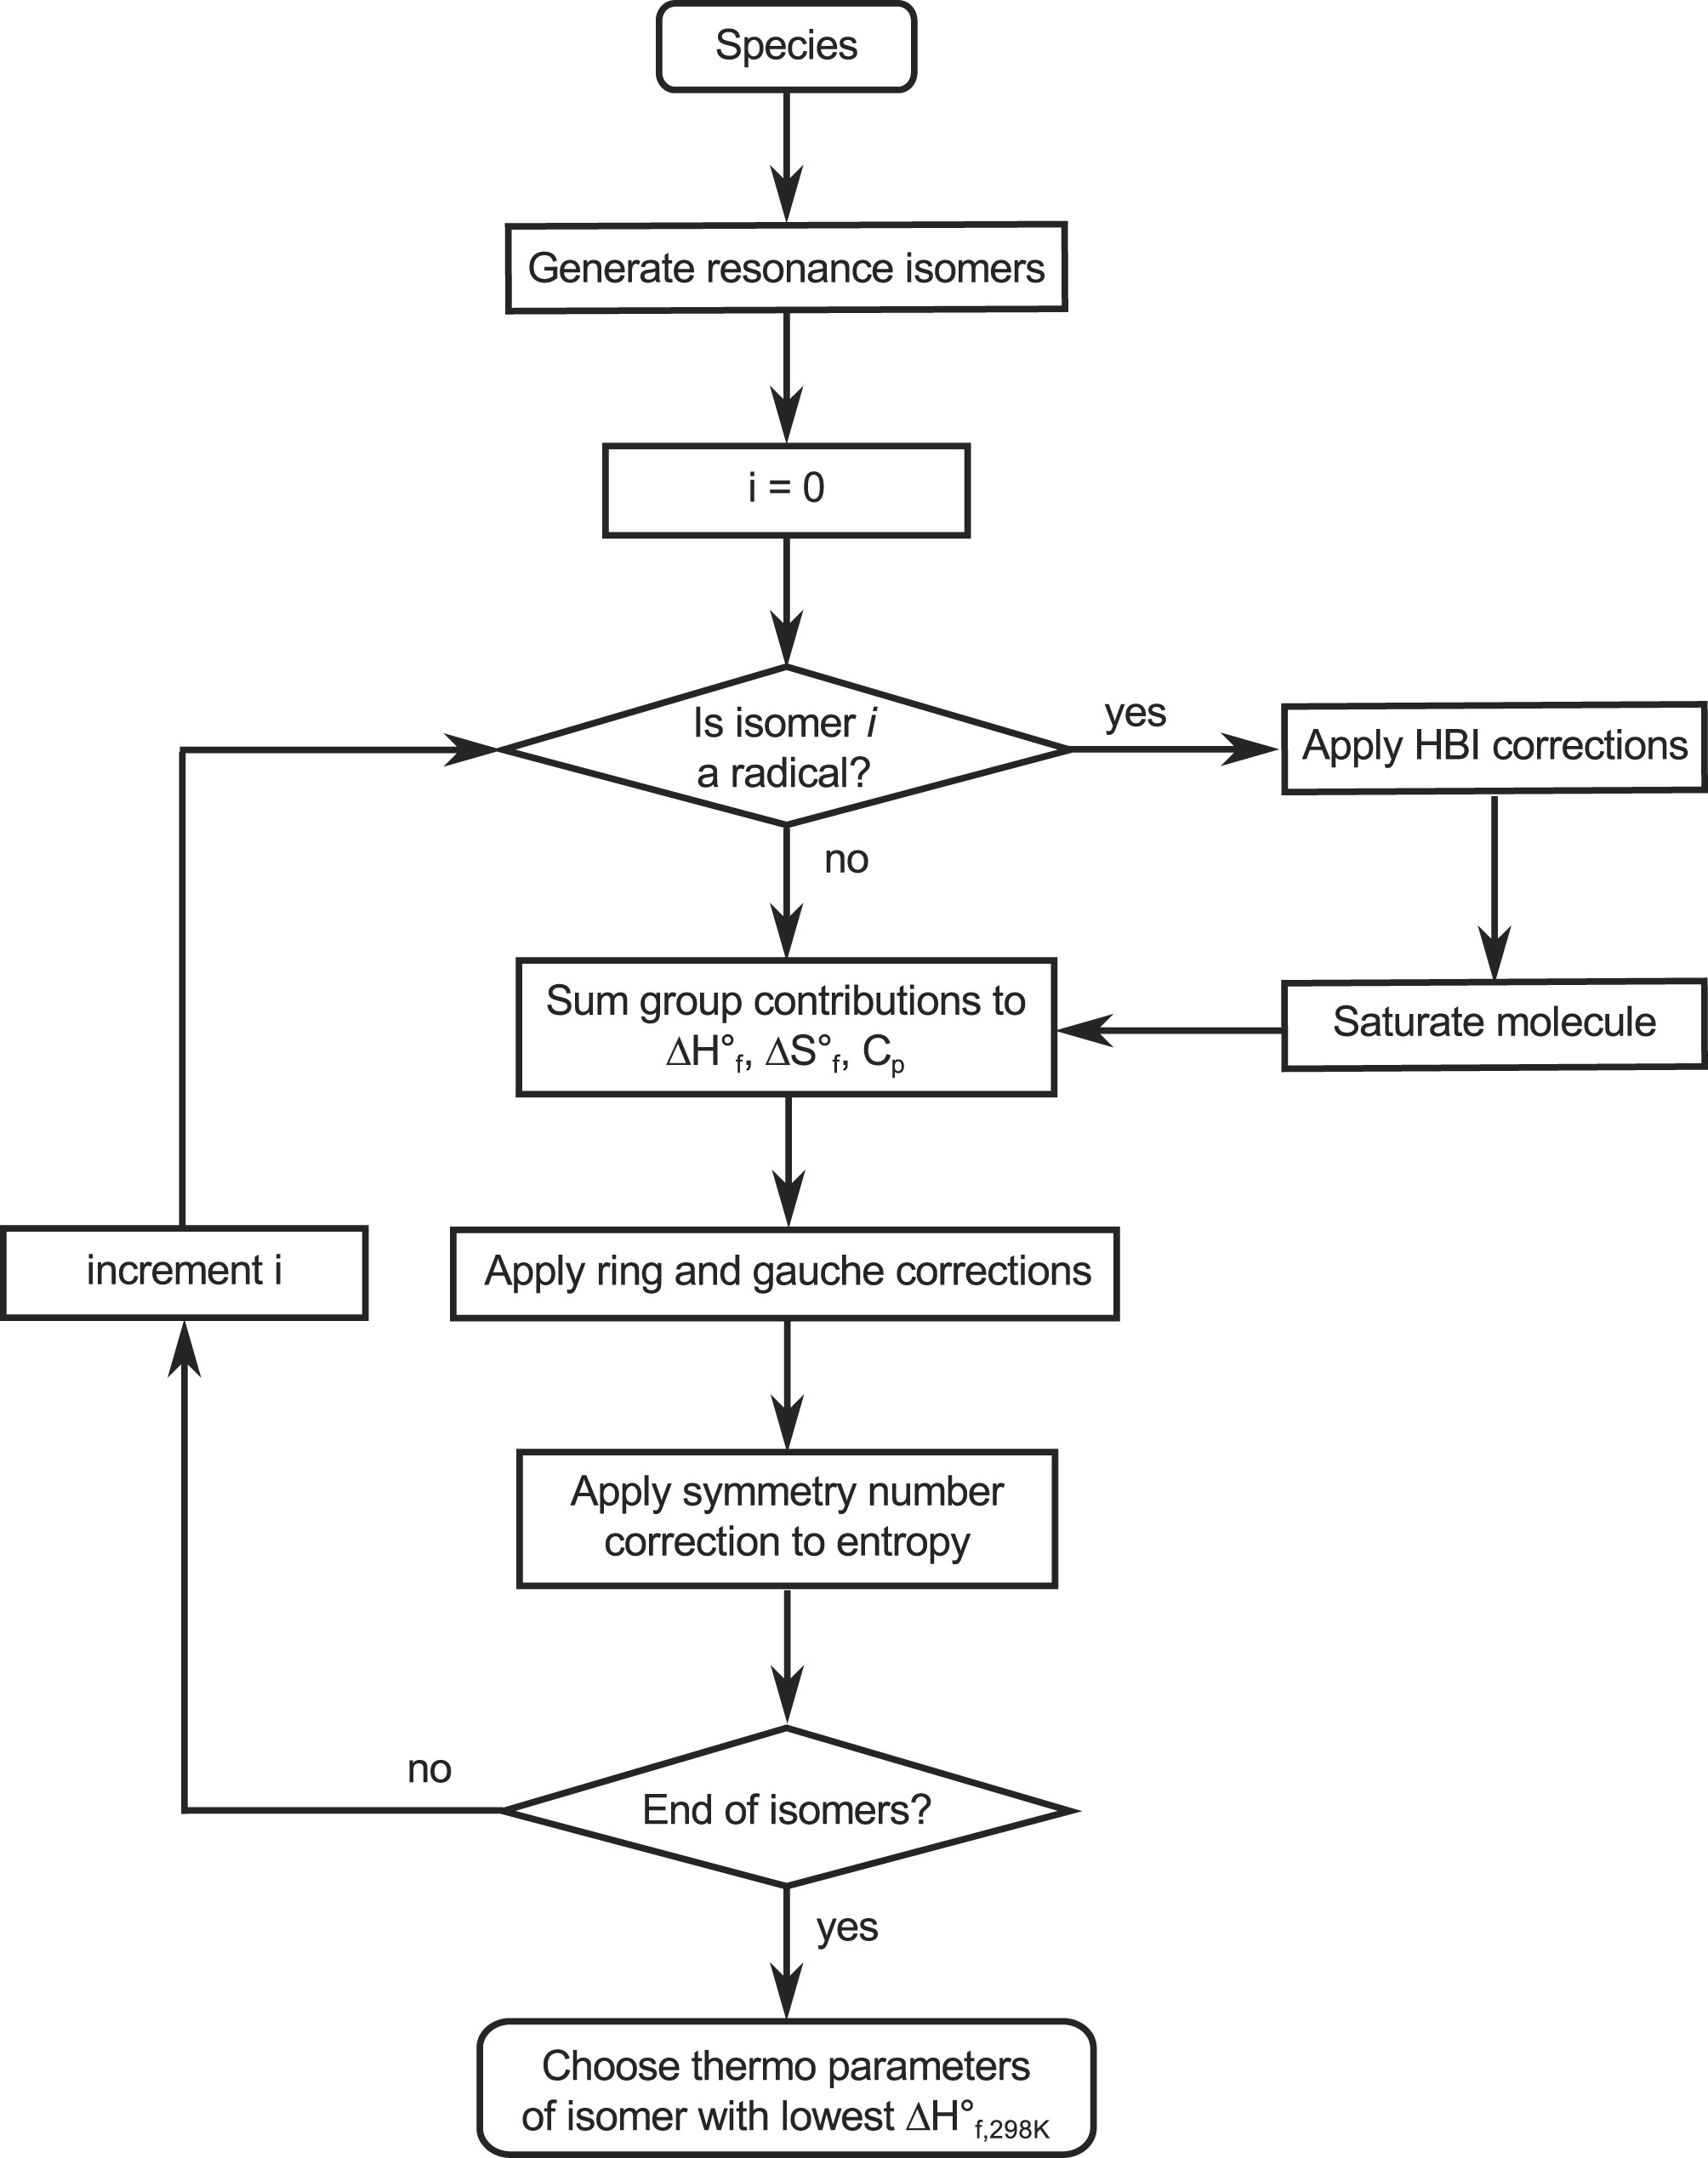
\includegraphics[scale=0.85]{images/tree-structure.jpg}
     \caption{RMG group-additivity thermodynamic parameter estimation algorithm \cite{Gao2016ReactionMechanisms}}
     \label{fig:tree}
 \end{figure}
 This entire process is done for before symmetry checks are applied to the total symmetry number of $\sigma$ bond correction at the entropy of formation.
\begin{equation}
    S^{\circ}=S_{GA}^{\circ}-R\ln\sigma
\end{equation} 
where, $S^{\circ}$ represents the standard corrected entropy of formation at 298K and $S_{GA}^{\circ}$ represents the group additivity standard entropy of formation at 298K, R is the gas constant. In fig.\ref{fig:tree} shows the entire algorithm followed for group-additivity thermodynamic estimation
 
 
 
 
 \subsection{RMG Kinetic Estimation}
 RMG is able to generate elementary reactions based on its library database of 45 reaction families of species. Each reaction family has a series of templates by which the reactive sites are identified as well as which reaction recipe to follow in order for bond connectivity to change as reactions proceed from reactants to products. Another set of hierarchical tree is used for rate estimates, assigning kinetics between reaction sites based on the closest matching functional group. The list of RMG reaction families are shown in the appendix.
%  
 
 
 
 
 In RMG, the forward rate constants are well defined based on thermodynamic parameters in its library database. Since the equilibrium constant $K_{eq}$ is also known again based on the thermodynamic estimates, the reverse rate is then given as \begin{equation}
     k_r=\frac{k_f}{K_{eq}}
 \end{equation}


\subsection{Seed Mechanisms}
Seed mechanisms are reaction libraries of other kinetic models that are automatically added to the model generation in RMG. The user starts off using a seed mechanism so as to guide RMG in the specific species, that must be included in the core of the model as well as the rates used in the quantification of these species rather than RMG's own group-additivity methods. This practice is done when a specific species or set of rates must be included in the mechanism. For the GTL PRFs, multiple seed mechanisms were used in order to reproduce the bulk of the species found in the literature and controls the auto-ignition properties of the fuel.


\subsection{Reactors with Pressure Dependence}
Unimolecular reactions are reactions that occur alone as only one reactant is present. These reactions in the process of going from reactants to products, require sufficient energy to overcome the energy barrier. Since these reactions can occur via isomerization such as \reaction{A\rightleftharpoons B} as well as that of dissociation or association reactions where \reaction{A\rightleftharpoons B + C} For gas-phase reactions to occur, it must be due to collisions as known in the Kinetic Theory of Gases. Thus, there must be a collider gas or an increase in the pressure of the system. If the sole reactant is then excited to a higher energy state, it thus possesses sufficient energy to overcome the activation energy barrier. If that activated species is excited it is then denoted as \reaction{A^* \rightleftharpoons B^*} and \reaction{A^* \rightleftharpoons B + C} The activated species can thus be activated in one of the following ways:
\begin{enumerate}
    \item Chemical activation such that $A^*$ is the product of the association reaction \reaction{B + C \rightleftharpoons A^*}
    \item Thermal activation which occurs when a collider species usually inert transfers energy to the reacting species through bimolecular collision \reaction{A + M \rightleftharpoons A^* + M} where M is the inert gas
    \item Photoactivation where A* is the product of a photon absorption
    \reaction{A + h\nu \longrightarrow A^*}
\end{enumerate}

Once a species has been activated, multiple reactions then occur often competing between themselves - between isomerizations and bimolecular reactions and as they attain collisional stabilization or thermal deactivation, they form a network of unimolecular reactions. The dominant pathway depends on the relative rates of collision and the reactions, which is now a function of temperature and pressure. At higher pressures, the collision rate is fast and activated species tend to attain thermal deactivation (collisional stabilization) before further reactions occur, usually referred to as the high-pressure limit. Similarly, at lower pressures, the collision rates are low and more reactions of the species occur between dissociations and isomerizations  before collisional stabilization is attained. The region at which pressure-dependence begins to affect reactions varies with temperature and molecular size\cite{Wong2003TemperatureLimit} as seen in fig.\ref{fig:pdep}.

\begin{figure}[t]
    \centering
    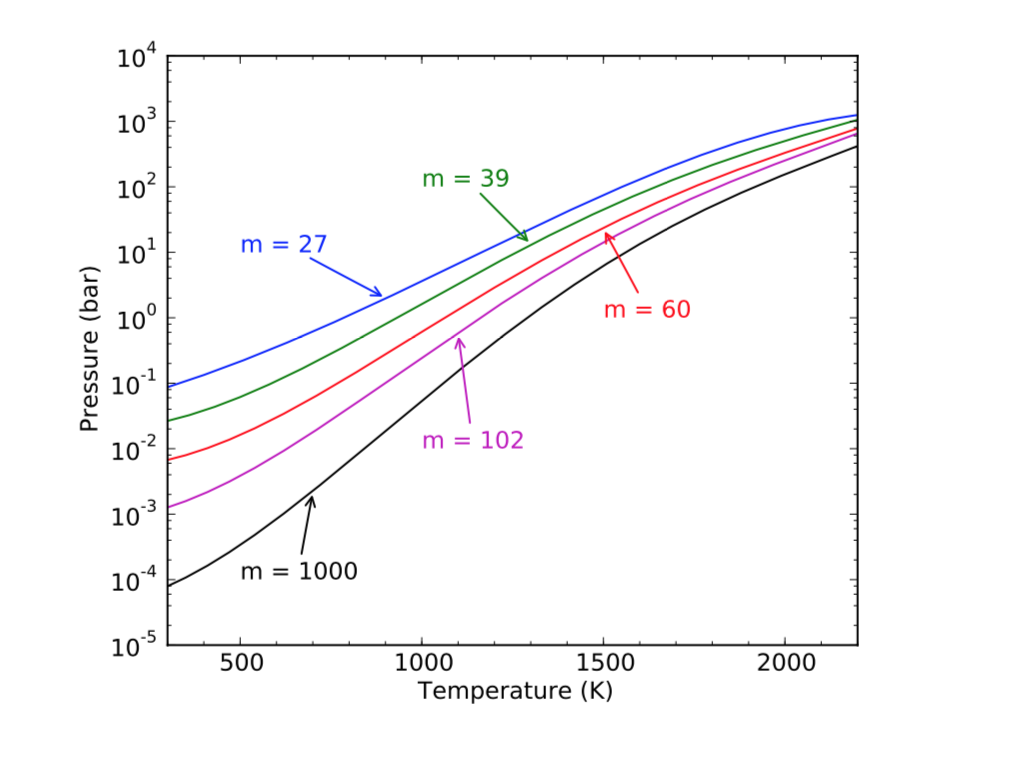
\includegraphics[scale=0.75, keepaspectratio]{images/pdep_limit.png}
    \caption{Plot of the switchover pressure - indicating the onset of pressure dependence - as a function of temperature and molecular size. The value $m\equiv N_{vib}+\frac{1}{2}N_{rot}$ represents a count of the internal degrees of freedom. Over a wide variety of conditions of practical interest, even very large molecules exhibit significant pressure dependence. \cite{Wong2003TemperatureLimit}}
    \label{fig:pdep}
\end{figure}
For the bulk of this work on all the PRFS of n-decane, iso-octane and n-propyl-cyclohexane, pressure dependence based on the guide of \cite{Wong2003TemperatureLimit} and fig.\ref{fig:pdep} was used to certify why pressure dependent models were necessary in building the GTL surrogates.

\vspace{1.5cm}

\subsection{Rate-based Algorithm and Filtering Reactions}
RMG makes use of the algorithm of Susnow et al \cite{Susnow1997Rate-BasedSystems} to decide which model species and reactions are included in the the core of the mechanism. The Algorithm as shown in the illustration of fig.\ref{fig:rmg_modelflux} with a grpahic illustration in fig.\ref{fig:rate-schematic}shows how the model generation process occurs and the decision tree for model move to core criteria. Since each model starts off with only user defined set of initial conditions as well as convergence criteria (termination condition for model generation to stop), the model termination can be a set of conditions such terminationtime, species conversion and terminationrateratio.
\begin{figure}[ht]
    \centering
    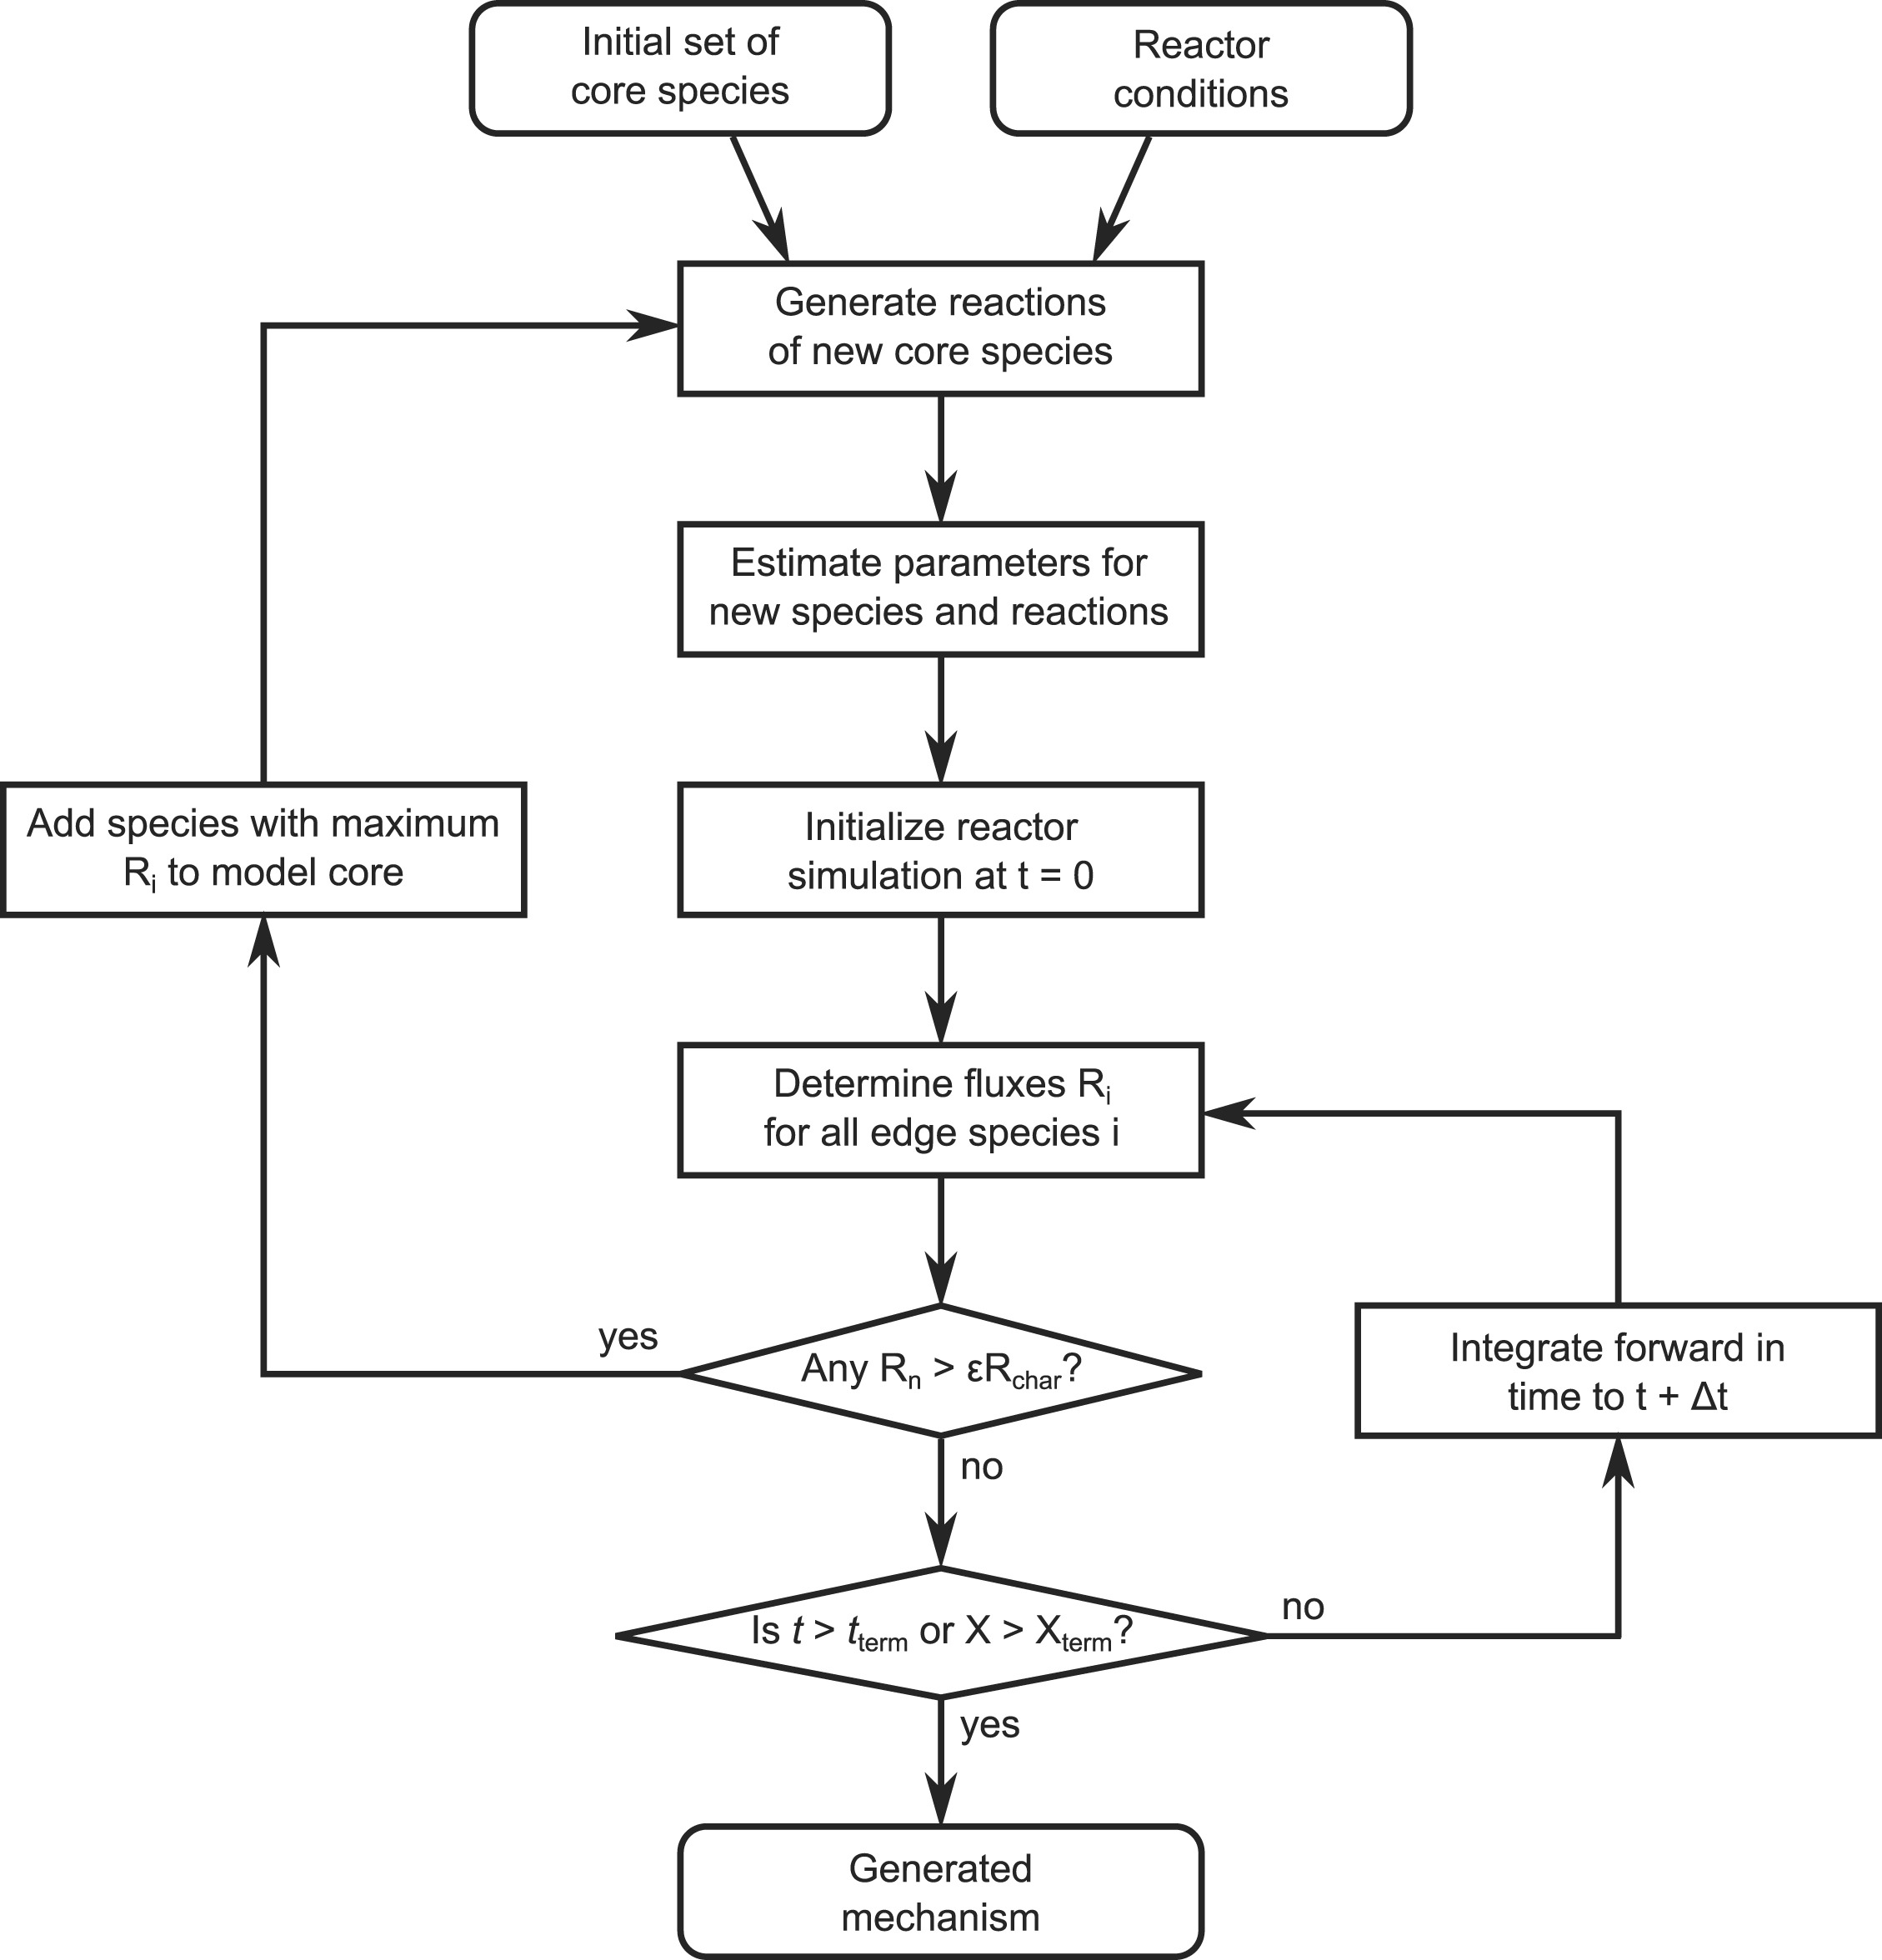
\includegraphics{images/rmg_model_flux.jpg}
    \caption{Flowchart of the Susnow et al\cite{Susnow1997Rate-BasedSystems} model rate algorithm as implemented in RMG}
    \label{fig:rmg_modelflux}
\end{figure}

Since RMG typically generates models at well defined and set temperature and pressure reactors, the need to generate models that span a wide range of temperatures and pressures is important. Rather than set a fixed constant temperature and pressure condition for reactors, RMG has a unique capability of doing a range based reactor. This means that RMG takes in various reactor conditions of temperature, pressure and species concentrations, using a weighted stochastic grid sampling algorithm, RMG samples the space of the range reactor conditions given based on the previous run conditions evaluated at the combination of the temperature pressure concentration pair. Each iteration is a grid of points spanning the reactor range where the grid has $20^N$ points and N is the number of dimensions.The grid values are normalized to one and a grid is chosen with a probability that is equal to the normalized objective function. A random step of maximum length is taken at a $\sqrt{2}/2$ times the distance between each grid point to the point of interest where the sampling starts. With this algorithm, RMG is able to then generate models at reactor range conditions and thereby reduce the computational cost of running at various points. 

\begin{figure}[ht]
    \centering
    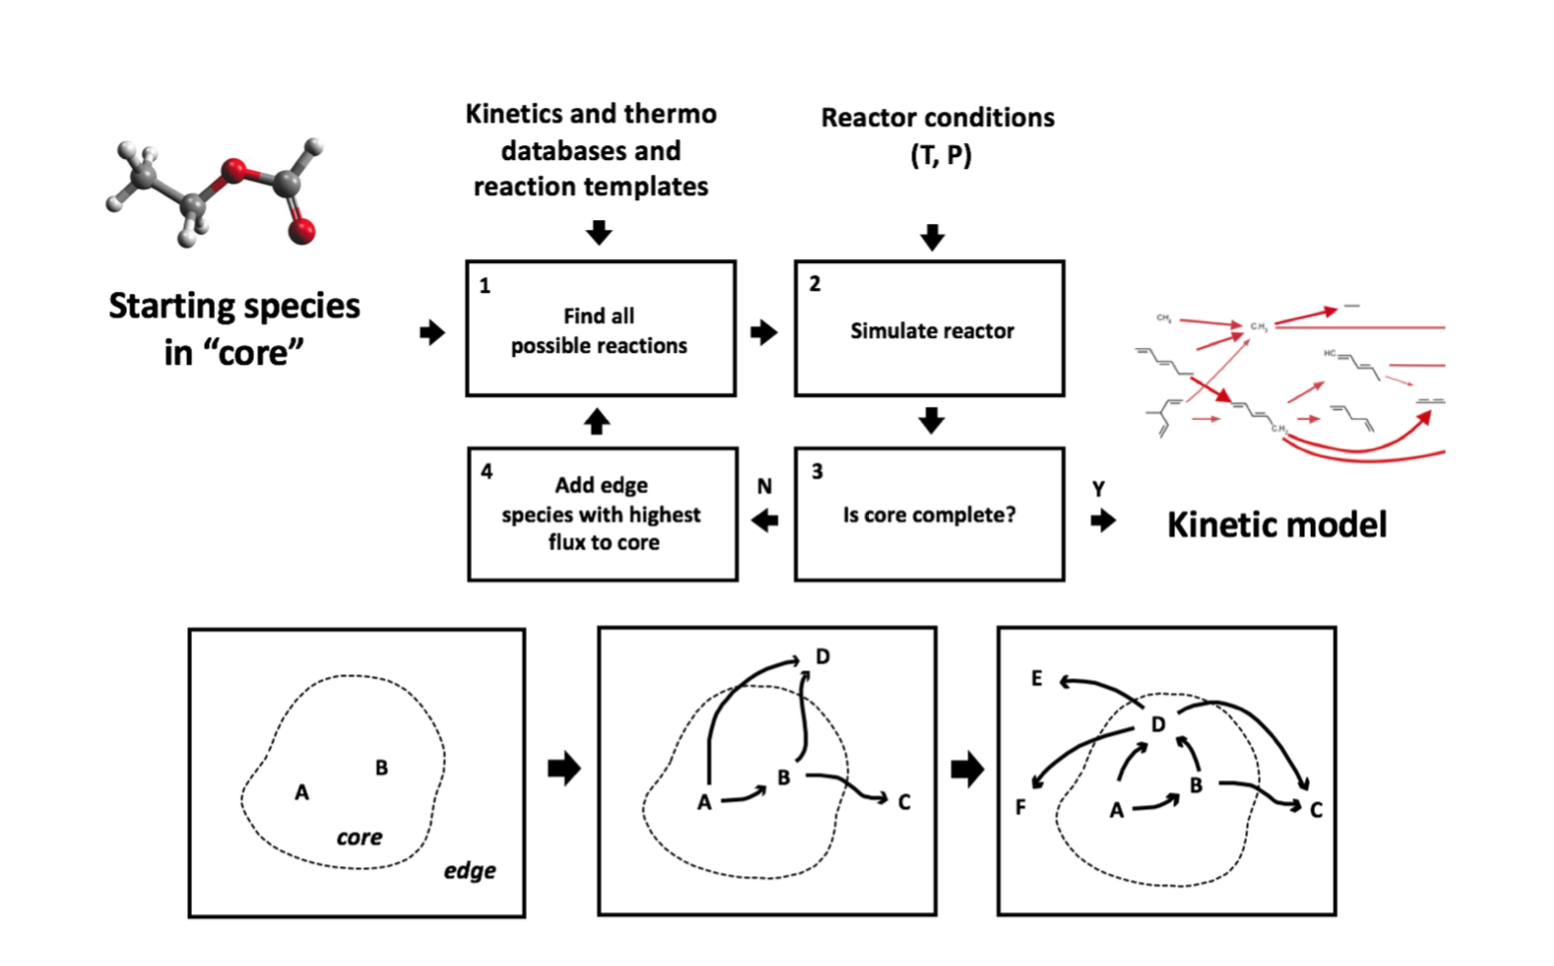
\includegraphics[scale=0.45,keepaspectratio]{images/rate-schematic.png}
    \caption{Schematic of the rate-based enlarging algorithm as described by Susnow et al\cite{Susnow1997Rate-BasedSystems} and illustration from RMG team\cite{Gao2016ReactionMechanisms}}
    \label{fig:rate-schematic}
\end{figure}


This range reactor model was applied on all PRF models of the GTL fuel surrogate (n-decane, iso-octane and propyl-cyclohexane) as well as the mix of all species of the PRFs in the starting input file.


\newpage

\section{Model Generation of PRFs in RMG}

Since RMG has all the capabilites needed to fully generate a detailed chemical kinetic mechanism, the PRFs of this GTL fuel blend was constructed using the aforementioned strategies outlined in Table \ref{tab:PRF_table}. 


\begin{table}[ht]
\arrayrulecolor[HTML]{DB5800}
\caption{Summary of the RMG input parameters in the database block for the model generation of PRFs: n-decane, iso-octane, n-propyl-cyclohexane and the GTL blend with input species}
\centering
\begin{adjustbox}{width=1\textwidth}
\small
\begin{tabular}{ p{5cm} p{5cm} p{5cm} p{5cm} p{5cm} }
    \hline
    \rowcolor{lightgray} \multicolumn{5}{|c|}{RMG PRF Input File Options} \\
    \hline
    Model Syntax  & n-decane & iso-octane & n-propyl-cyclohexane & GTL model blend with all PRF species added \\
    \hline
    thermoLibraries used \\
    - & BurkeH2O2 & BurkeH2O2 & BurkeH2O2 & BurkeH2O2 \\
    - & Klippenstein\textunderscore Glarborg2016 & Klippenstein\textunderscore Glarborg2016 & Klippenstein\textunderscore Glarborg2016 & Klippenstein\textunderscore Glarborg2016 \\
    - & CurranPentane & CurranPentane & CurranPentane & CurranPentane \\
    - & FFCM1(-) & FFCM1(-) & FFCM1(-) & FFCM1(-) \\
    - & primaryThermoLibrary & primaryThermoLibrary & JetSurF2.0 & JetSurF2.0 \\
    - & thermo\textunderscore DFT\textunderscore CCSDTF12\textunderscore BAC &  thermo\textunderscore DFT\textunderscore CCSDTF12\textunderscore BAC & primaryThermoLibrary & primaryThermoLibrary \\
    - & DFT\textunderscore QCI\textunderscore thermo & DFT\textunderscore QCI\textunderscore thermo & thermo\textunderscore DFT\textunderscore CCSDTF12\textunderscore BAC & thermo\textunderscore DFT\textunderscore CCSDTF12\textunderscore BAC \\
    - & CBS\textunderscore QB3\textunderscore 1dHR & CBS\textunderscore QB3\textunderscore 1dHR & DFT\textunderscore QCI\textunderscore thermo & DFT\textunderscore QCI\textunderscore thermo \\
    - & - & - & CBS\textunderscore QB3\textunderscore 1dHR & CBS\textunderscore QB3\textunderscore 1dHR \\
    \hline
    reactionLibraries used \\
    - & CurranPentane & CurranPentane & violator\textunderscore fixes\textunderscore 500-1500K & JetSurF2.0 \\
    - & FFCM1(-) & FFCM1(-) & JetSurF2.0 & FFCM1(-) \\
    - & combustion\textunderscore core/version5 & combustion\textunderscore core/version5 & CurranPentane & combustion\textunderscore core/version5 \\
    - & - & - & FFCM1(-) & - \\
    - & - & - & combustion\textunderscore core/version5 & - \\
    \hline
    seedMechanisms \\
    - & BurkeH2O2inN2 & BurkeH2O2inN2 & BurkeH2O2inN2 & BurkeH2O2inN2 \\
    - & Klippenstein\textunderscore Glarborg2016 & BurkeH2O2inArHe & Klippenstein\textunderscore Glarborg2016 & Klippenstein\textunderscore Glarborg2016 \\
    - & \ce{C2H4+O\textunderscore Klipp2017} & \ce{C2H4+O\textunderscore Klipp2017} & \ce{C2H4+O\textunderscore Klipp2017} & \ce{C2H4+O\textunderscore Klipp2017} \\
    - & - & Klippenstein\textunderscore Glarborg2016 & - & - \\
    \hline 
    kineticDepositories used \\
    - & training & training & training & training \\
    \hline
    kineticsFamilies used\\
    - & default & default & default & default \\
    \hline
    kineticsEstimator used\\
     - & rate rules & rate rules & rate rules & rate rules \\
    \hline
    \end{tabular}
    \end{adjustbox}
    
    \label{tab:PRF_table1}
    
\end{table}

The additional set of options in RMG, which aided in the construction of the PRFs as well as the GTL mixture blend was done to enable computational efficiency as well as proximity to the real GTL fuel blend as described in \cite{Dagaut2014}.


\begin{table}
\arrayrulecolor[HTML]{DB5800}
\caption{Summary of the RMG input parameters in the simple reactor 1-2 block for the model generation of PRFs: n-decane, iso-octane, n-propyl-cyclohexane and the GTL blend with input species}
\centering
\begin{adjustbox}{width=1\textwidth}
\begin{tabular}{ p{5cm} p{5cm} p{5cm} p{5cm} p{6cm} }
    \hline
    \rowcolor{lightgray} \multicolumn{5}{|c|}{RMG PRF Input File Options} \\
    \hline
    Model Syntax  & n-decane & iso-octane & n-propyl-cyclohexane & GTL model blend with all PRF species added \\
    \hline
    SimpleReactor 1 Conditions \\ 
    \hline
    temperature range & 550K - 1500K & 550K - 1500K & 550K - 1500K & 550K - 1500K \\
    pressure range & 1 bar - 40 bar & 1 bar - 40 bar & 550K - 1500K & 550K - 1500K \\
    nSims & 10 & 30 & 30 & 40 \\
    initial Mole Fractions  \\
    Fuel & \[\frac{0.000983928}{2} - 0.000983928\times 2\] & \[\frac{0.0165224}{2} - 0.0165224\times 2\]   & \[\frac{0.015748}{2} - 0.015748\times 2\] &  \begin{tabular}{ c }
         n\ce{C_{10}H_{22}}: $\frac{0.000577}{2} - 0.000577\times 2$  \\
         i\ce{C_8H_{18}}:   $\frac{0.000332}{2} - 0.000332\times 2$ \\
         n\ce{C_9H_{18}}: $\frac{0.000091}{2} - 0.000091\times 2$ \\
                                                            \end{tabular}\\ 
    \ce{N2} & 0.983765 &  0.776947 & 0.787402 & 0.787402 \\
    \ce{O2} & 0.0152509 & 0.20653 & 0.19685 & 0.19685 \\
    terminationConversion & - & - & - & \begin{tabular}{ c } 
          n\ce{C_{10}H_{22}}: 0.90\\
          i\ce{C_8H_{18}}: 0.90 \\
          n\ce{C_9H_{18}}: 0.99 \\
    \end{tabular}\\
    terminationTime & 1.0 s & 40.0 s & 40.0 s & 40.0 s \\
    terminationRateRatio & 0.01 & 0.01 & 0.05 & 0.01 \\
    \hline
     SimpleReactor 2 Conditions \\
     \hline
    temperature range & 550K - 800K & 550K - 800K & 550K - 800K & 550K - 800K \\
    pressure range  & 1 bar - 40 bar & 1 bar - 40 bar & 1 bar - 40 bar & 1 bar - 40 bar \\
    nSims & 10 & 60 & 60 & 60 \\
     initial Mole Fractions & \[\frac{0.000983928}{2} - 0.000983928\times 2\]  & \[\frac{0.0165224}{2} - 0.0165224\times 2\] & \[\frac{0.015748}{2} - 0.015748\times 2\]  & \begin{tabular}{ c }
         n\ce{C_{10}H_{22}}: $\frac{0.000577}{2} - 0.000577\times 2$  \\
         i\ce{C_8H_{18}}:   $\frac{0.000332}{2} - 0.000332\times 2$ \\
         n\ce{C_9H_{18}}: $\frac{0.000091}{2} - 0.000091\times 2$ \\
    \end{tabular}\\  
    \ce{N2} & 0.983765 &  0.776947 & 0.787402 & 0.787402 \\
    \ce{O2} & 0.0152509 & 0.20653 & 0.19685 & 0.19685 \\
    terminationConversion & - & - & - & \begin{tabular}{ c }
          n\ce{C_{10}H_{22}}: 0.99\\
          i\ce{C_8H_{18}}: 0.99 \\
          n\ce{C_9H_{18}}: 0.99 \\
    \end{tabular}\\
    terminationTime & 1.0 s & 40.0 s & 40.0 s & 40.0 s \\
    terminationRateRatio & 0.01 & 0.01 & 0.05 & 0.05 \\
    \hline
    \end{tabular}
    \end{adjustbox}
    
    \label{tab:PRF_table2}
\end{table}
    
\begin{table}
\arrayrulecolor[HTML]{DB5800}
\caption{Summary of the RMG input parameters in the simple reactor 3-4 block and option for pressure dependence for the model generation of PRFs: n-decane, iso-octane, n-propyl-cyclohexane and the GTL blend with input species}
\centering
\begin{adjustbox}{width=1\textwidth}
\begin{tabular}{ p{5cm} p{5cm} p{5cm} p{5cm} p{6cm} }    
    
    \hline 
    \rowcolor{lightgray} \multicolumn{5}{|c|}{RMG PRF Input File Options} \\
    \hline
    Model Syntax  & n-decane & iso-octane & n-propyl-cyclohexane & GTL model blend with all PRF species added \\
    \hline \\
    SimpleReactor 3 Conditions               \\ 
    \hline \\
    temperature range & 550K - 700K & 550K - 700K & 550K - 700K & 550K - 700K \\
    pressure range  & 1 bar - 40 bar & 1 bar - 40 bar & 1 bar - 40 bar & 1 bar - 40 bar \\
    nSims & 10 & 60 & 60 & 60 \\
    initial Mole Fractions & \[\frac{0.000983928}{2} - 0.000983928\times 2\]  & \[\frac{0.0165224}{2} - 0.0165224\times 2\] & \[\frac{0.015748}{2} - 0.015748\times 2\]  & \begin{tabular}{ c }
         n\ce{C_{10}H_{22}}: $\frac{0.000577}{2} - 0.000577\times 2$  \\
         i\ce{C_8H_{18}}:   $\frac{0.000332}{2} - 0.000332\times 2$ \\
         n\ce{C_9H_{18}}: $\frac{0.000091}{2} - 0.000091\times 2$ \\
    \end{tabular}\\  
    \ce{N2} & 0.983765 &  0.776947 & 0.787402 & 0.787402 \\
    \ce{O2} & 0.0152509 & 0.20653 & 0.19685 & 0.19685 \\
    terminationConversion & - & - & - & \begin{tabular}{ c }
          n\ce{C_{10}H_{22}}: 0.99\\
          i\ce{C_8H_{18}}: 0.99 \\
          n\ce{C_9H_{18}}: 0.99 \\
    \end{tabular}\\ 
    terminationTime & 1.0 s & 40.0 s & 40.0 s & 40.0 s \\
    terminationRateRatio & 0.01 & 0.01 & 0.05 & 0.05 \\
    \hline \\
    {SimpleReactor 4 Conditions} \\
    \hline \\
    temperature range & 550K - 600K & 550K - 600K & 550K - 600K & 550K - 600K \\
    pressure range  & 1 bar - 40 bar & 1 bar - 40 bar & 1 bar - 40 bar & 1 bar - 40 bar \\
    nSims & 10 & 60 & 60 & 60 \\
    initial Mole Fractions & \[\frac{0.000983928}{2} - 0.000983928\times 2\]  & \[\frac{0.0165224}{2} - 0.0165224\times 2\] & \[\frac{0.015748}{2} - 0.015748\times 2\]  & \begin{tabular}{ c }
         n\ce{C_{10}H_{22}}: $\frac{0.000577}{2} - 0.000577\times 2$  \\
         i\ce{C_8H_{18}}:   $\frac{0.000332}{2} - 0.000332\times 2$ \\
         n\ce{C_9H_{18}}: $\frac{0.000091}{2} - 0.000091\times 2$ \\
    \end{tabular}\\  
    \ce{N2} & 0.983765 &  0.776947 & 0.787402 & 0.787402 \\
    \ce{O2} & 0.0152509 & 0.20653 & 0.19685 & 0.19685 \\
    terminationConversion & - & - & - & \begin{tabular}{ c }
          n\ce{C_{10}H_{22}}: 0.99\\
         i\ce{C_8H_{18}}: 0.99 \\
          n\ce{C_9H_{18}}: 0.99 \\
    \end{tabular}\\
    terminationTime & 1.0 s & 40.0 s & 40.0 s & 40.0 s \\
    terminationRateRatio & 0.01 & 0.01 & 0.05 & 0.05 \\
    \hline
    Pressure Dependence & modified strong collision & modified strong collision & modified strong collision & modified strong collision \\
    \hline
    \end{tabular}
    \end{adjustbox}
    
    \label{tab:PRF_table3}
\end{table}


In addition to the database of the PRFs, the model generation of the GTL fuel blended surrogate, was achieved using two main techniques:
\begin{enumerate}
    \item Primary construction of the detailed mechanism of each primary reference fuel (PRF) validated at different temperature and pressure conditions. Then concatenation (merging) of the three-component fuel blend.
    \item Cross reaction of the primary reference fuel input species at specific species concentrations.
\end{enumerate}

The first method used for the concatenated GTL fuel surrogate is described in more detail in the subsequent chapters with an illustration in fig.\ref{fig:gtl-surrogate} using RMG's inbuilt mergemodel script  that takes in the mechanism that include both the thermodynamics of the model as well as the reactions, while the species identifier was added as an argument alongside the transport file for the flame analysis.


\begin{figure}
\hspace*{-2cm}
    \centering
    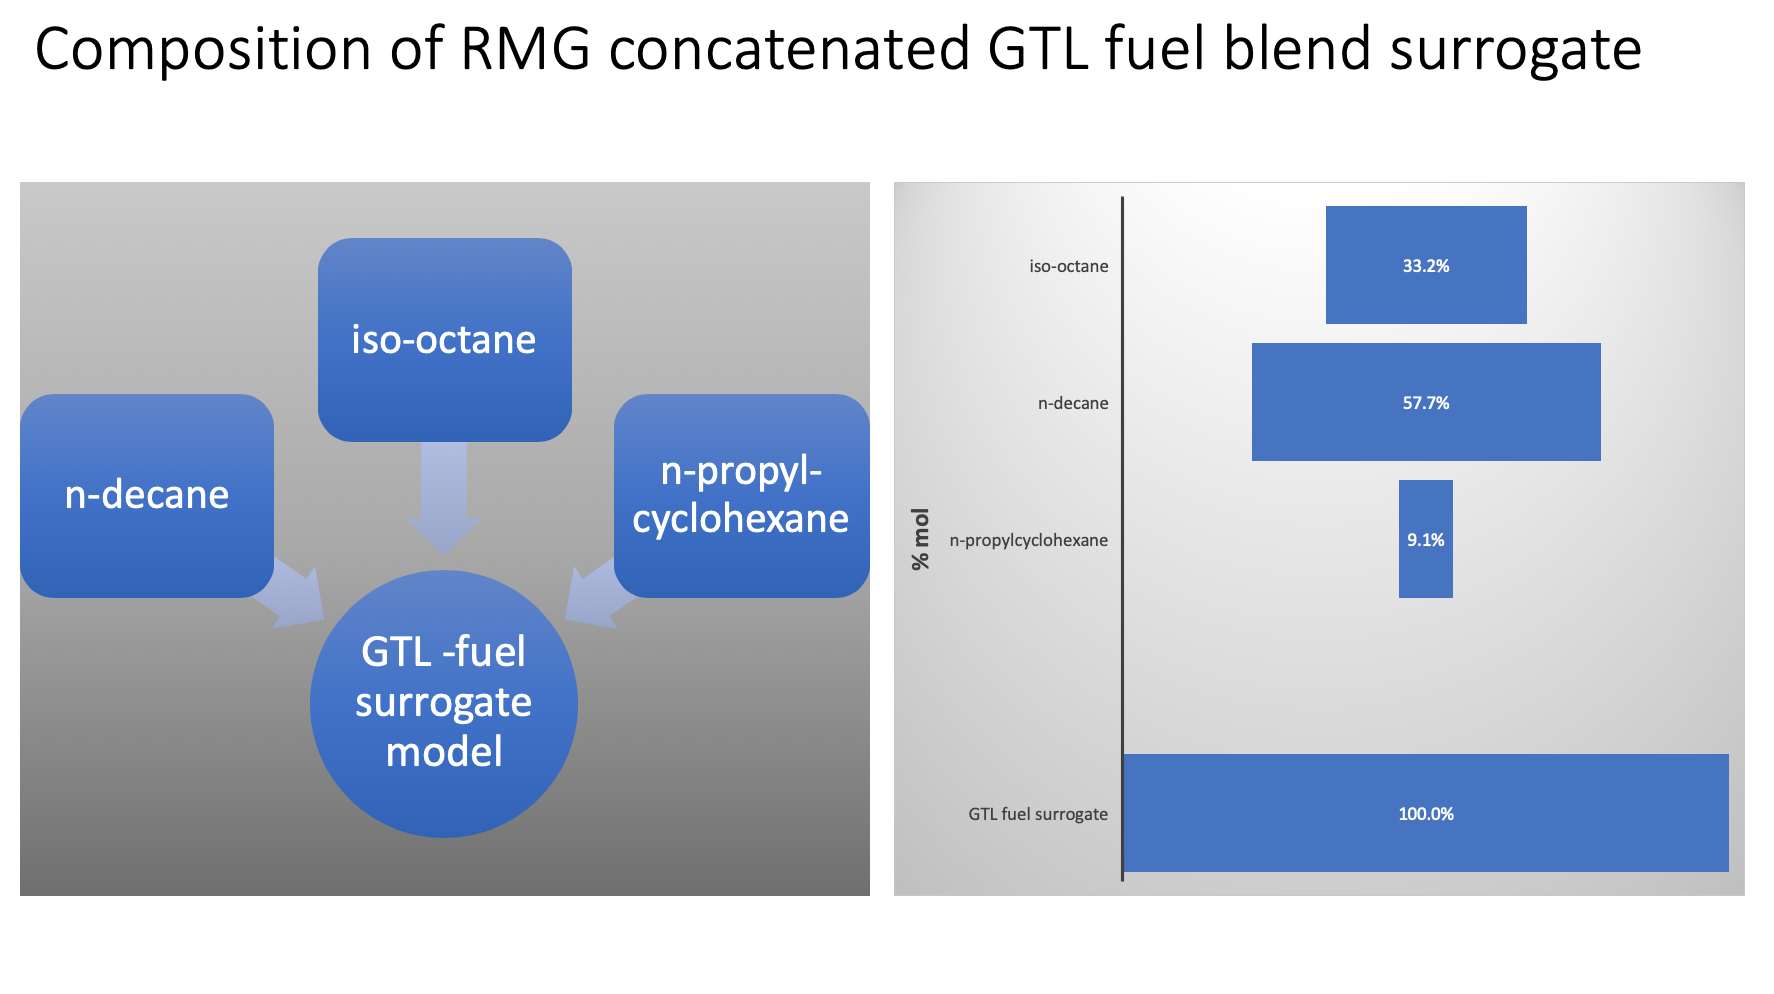
\includegraphics[scale=0.5,keepaspectratio]{images/GTL-Constituents.png}
    \caption{Composition of RMG concatenated GTL fuel surrogate model from the detailed mechanisms of n-decane, iso-octane and propyl-cyclohexane}
    \label{fig:gtl-surrogate}
\end{figure}


The second method involves a GTL fuel surrogate model that is constructed with all input species added from the onset such that cross-reactions are allowed shown in fig.\ref{fig:gtl_cross_rxn}. 

\begin{figure}
\hspace*{-2cm}
    \centering
    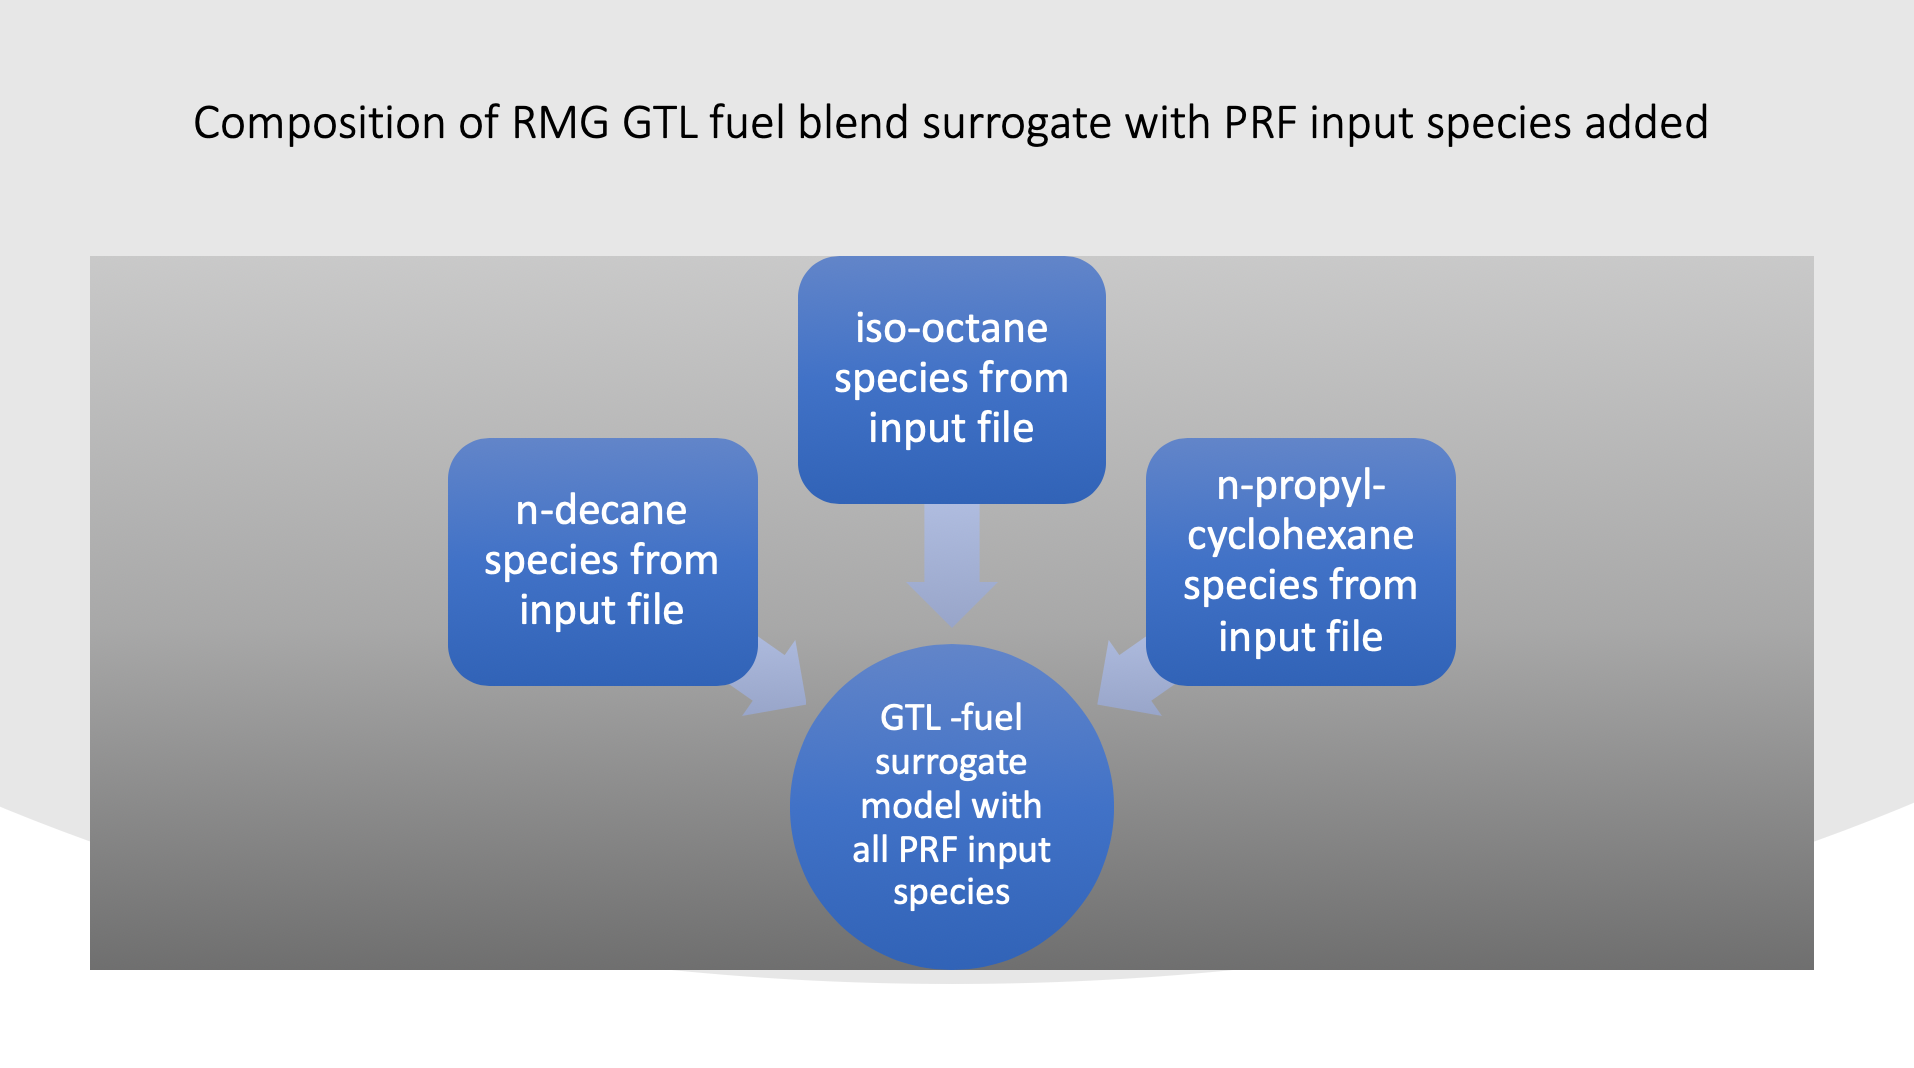
\includegraphics[scale=0.5, keepaspectratio]{images/GTL-cross-rxn.png}
    \caption{Illustration of GTL fuel surrogate model from the input species of PRFs}
    \label{fig:gtl_cross_rxn}
\end{figure}